Travlendar+ is a service based on a mobile application and a web application.
\newline
\newline
The user simply has to create events that he wants to insert into his schedule; the application will then organize travels in order to reach locations in the best way, correctly inserting them within the daily schedule and notifying eventual overlappings. \newline
The user can modify the schedule with any feasible combination of added events and can specify different types of preferences on travel means, so the system can plan the trip according to his personal needs.
\newline
\newline
The principal goal of Travlendar+ is to save time, both in the construction of the schedule and in the traveling between events.
The main functionality of the system is to control the user's daily flow of events, helping him optimizing his time and making sure that all his preferences and constraints are respected.
Integration with external transport means providers is also offered, allowing the user to buy tickets and locate travel means without exiting the app.
\newline

\subsection{World and shared phenomena}
This is an overview of the world in which Travlendar+ is intended to exist: the system aims to plan events and appointment of the user in a way that allows him to take part in each of them. So the world is made of entity related to travel. 
\newline
\newline
Shared phenomena allow the user to achieve his goals and affect both user and system behaviours:
\begin{itemize}
	\item Arrange trips and create schedules are phenomena controlled by the machine and observed by the world. 
	\item Define constraints and create events instead are phenomena controlled by the world and observed by the machine.
\end{itemize}
The machine encloses the set of functions used to perform the different tasks. These items are not visible in the world.
\newline
\begin{figure} [h]
\centering
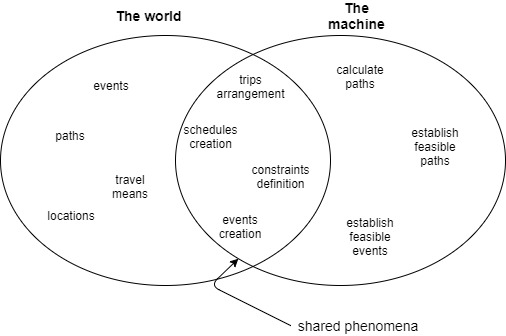
\includegraphics[scale=0.6]{shared_phenomena.jpg}
\end{figure}
